\noindent
\textbf{CS4268 AY2025-26 Sem 2}
\\
\noindent
Lecturer: Divesh Aggarwal
\hfill
Lecture 10                      %%% FILL IN LECTURE NUMBER HERE
\hfill
Date: March 26, 2026          %%% FILL IN LECTURE DATE HERE


\noindent
\rule{\textwidth}{1pt}

\medskip


\section{Grover's Search Algorithm}

Today is on search and Grover's algorithm. The main theme is that quantum interference can be exploited to amplify the amplitude on the marked states, ultimately giving a quadratic speedup over classical black-box search.

\paragraph{Problem.} We want to search for (any) one of $M$ marked elements among $N$ elements. Given a Boolean function $f: [N]=\{0,1,\dots,N-1\} \longrightarrow \{0,1\}$. $f(x)=1$ if $x$ is one of those marked elements, otherwise $f(x)=0$.

\paragraph{Classical Solution.} Classically, this search problem requires linear query complexity. For a deterministic algorithm, in the worst case we may need to inspect all $N$ items before finding a marked one, so the worst-case query complexity is $N$. For a randomized algorithm, if we query $k$ uniformly random items, the probability of missing every marked element is approximately $(1-M/N)^k$, assuming $M \ll N$. Thus if we require that we find (at least) a solution with probability as least $1-\varepsilon$, then we have $1-(1-\frac{M}{N})^k \approx kM/N \geq 1-\varepsilon$, i.e. for a fixed error margin we need $k=\Omega(N/M)$ queries to solve the problem. 

\paragraph{Grover's Algorithm.} Grover's algorithm solves this search problem using $\mathcal{O}(\sqrt{N/M})$ oracle queries, thus giving a \textit{quadratic speedup in query complexity}. Grover search is a two-step procedure repeated multiple times: first the oracle flips the phase of the marked states, and then a second operation reflects again about the uniform superposition. Together these move amplitude from unmarked states to marked states.

\begin{algorithm}
    \caption{Grover's Algorithm}
    %\label{algo:TGD}
    \begin{algorithmic}[1]
    \Require Oracle $O_f$ to implement $f$ unitarily, where $f$ specifies the solutions.
    \State Initialize the state $\ket{0^n}\ket{0}$.
    \State Apply $H^{\otimes n}$ to the $n$ work qubits and $HX$ to the ancillary qubit:
    \[
        (H^{\otimes n} \otimes HX)\ket{0^n}\ket{0} = \frac{1}{\sqrt{2^n}}\sum_{x=0}^{2^n-1} \ket{x}\ket{-}.
    \]
    \State Apply the Grover operator $G=H^{\otimes n}(2\ketbra{0^n}{0^n}-I)H^{\otimes n}O_f$. Iterate $k = \left\lceil \frac{\pi}{4}\sqrt{\frac{N}{M}} \right\rceil$ times:
    \[
        G^k \left( \frac{1}{\sqrt{2^n}}\sum_{x=0}^{2^n-1} \ket{x} \right) = \alpha \left( \frac{1}{\sqrt{N-M}} \sum_{x \in A} \ket{x} \right) + \beta \left( \frac{1}{\sqrt{M}} \sum_{x \in B} \ket{x} \right)
    \]
    where $|\alpha| \ll 1$, $|\beta| \approx 1$. (Ancillary qubit suppressed.)
    \State Measure the $n$ work qubits.
    \Ensure $x \in B$ (the solution set) with high probability.
    \end{algorithmic}
\end{algorithm}

\begin{figure}[h]
    \label{GroverCircuit}
    \centering
    \begin{quantikz}[wire types = {b},classical gap=0.1cm, column sep=0.3cm]
    \lstick{$\ket{0^n}$} && \gate{H^{\otimes n}} \slice{} & \gate[2]{G} & \gate[2]{G} & \midstick[2,brackets=none]{$\cdots$} & \gate[2]{G} & \gate[2]{G} \slice{} && \meter{}\\
    \lstick{\text{Ancilla}\quad$\ket{0}$} & \gate{X} & \gate{H} &&&&&&& \rstick{$\ket{-}$}
    \end{quantikz}
    \caption{Quantum circuit implementing Grover's algorithm.}
    %\label{fig:enter-label}
\end{figure}

\begin{figure}[h]
    \centering
    \begin{quantikz}[wire types = {b},classical gap=0.1cm, column sep=0.3cm]
    & \gate[2]{G} & \midstick[2,brackets=none]{=} & \gate[2]{O_f} & \gate{H^{\otimes n}} & \gate{2\ketbra{0^n}{0^n}-I} & \gate{H^{\otimes n}} &\\ 
    &&&&&&&
    \end{quantikz}
    \caption{The Grover Operator.}
\end{figure}

\paragraph{Analysis of Grover's Algorithm.} 

\begin{enumerate}
    \item First let
    \[
        \ket{\psi}=\frac{1}{\sqrt{2^n}}\sum_{x=0}^{2^n-1}\ket{x}
    \]
    denote the uniform superposition obtained after the initial Hadamards.
    
    \item The operator $2\ketbra{0^n}{0^n}-I$ is a conditional phase shift operator: upon its implementation every computational basis state except for $\ket{0^n}$ acquires a phase shift of $-1$. This is implemented using phase-kickback trick, where $f_{\text{pk}}(0^n)=0$ and $f_{\text{pk}}(x)=1$ for all $x \neq 0^n$. The Grover operator $G$ can then be written as
    \[
        G = (2\ketbra{\psi}{\psi}-I)O_f.
    \]
    After the preprocessing but before implementing $G$ (this stage is indicated by the dotted red line in Fig. \ref{GroverCircuit}), we have the initial state $\ket{\psi}$. Let us define the sets 
    \begin{align*}
        A &= \{x \in \{0,1\}^n \;|\; f(x)=0\}\\
        B &= \{x \in \{0,1\}^n \;|\; f(x)=1\}.
    \end{align*}
    (that is, $B$ is the set of solutions to the search problem) and their corresponding uniform superpositions
    \begin{align*}
        \ket{\alpha} &= \frac{1}{\sqrt{N-M}} \sum_{x \in A} \ket{x}\\
        \ket{\beta} &= \frac{1}{\sqrt{M}} \sum_{x \in B} \ket{x}.
    \end{align*}
    We can then rewrite
    \[
        \ket{\psi} = \sqrt{\frac{N-M}{N}}\ket{\alpha} + \sqrt{\frac{M}{N}}\ket{\beta}  
    \]
    as a vector in the 2D real subspace spanned by $\ket{\alpha}$ and $\ket{\beta}$. Note that $\braket{\beta}{\alpha}=0$. 
    
    Now comes the crucial part of the analysis: Since $O_f$ marks the solutions by introducing a phase shift of $-1$, we have $O_f(a\ket{\alpha}+b\ket{\beta}) = a\ket{\alpha}-b\ket{\beta}$, i.e. $O_f = 2\ketbra{\alpha}{\alpha}-1$ is also a reflection operator. Thus the Grover operator, being a composition of two reflection operators in $\mathbb{R}^2$, is also a rotation operator (see lemma below).

    \begin{lemma}
        In $\mathbb{R}^2$, the composition of two reflections is a rotation.
    \end{lemma}
    \begin{proof}
        Any reflection about the subspace spanned by the unit vector $v$ is given by $R_v = 2vv^T-1$. One can easily check (by evaluating the inner product) that for any arbitrary unit vector $w$, we have $\theta_{v,w} = \theta_{v,R_v(w)} = \frac{1}{2}\theta_{w,R_v(w)}$. Note that $\text{det}(R_v) = -1$ (where we have used the fact that the eigenvalues of the projector $vv^T$ are $1$ and $0$), as is expected for a reflection.

        Given arbitrary unit vectors $v,w$ defining the lines of reflection, we now show that their product is a proper rotation, i.e. it is orthogonal and has determinant $1$. Both proofs are straightforward. First we have $(2vv^T-1)(2vv^T-1) = 1$, thus $(R_vR_w)^T (R_vR_w) = I$; second we have $\text{det}(AB) = \text{det}(A)\text{det}(B)$, so $\text{det}(R_vR_w) = 1$.
    \end{proof}

    \begin{proposition}
        In the $\ket{\alpha},\ket{\beta}$ basis, the Grover operator is represented as
        \[
            G = 
            \begin{bmatrix}
                \cos \theta & -\sin \theta\\
                \sin \theta &
                \cos \theta
            \end{bmatrix},
        \]
        where $\theta$ is such that $\cos(\theta/2) = \sqrt{\frac{N-M}{N}}$ and $\sin(\theta/2) = \sqrt{\frac{M}{N}}$.
    \end{proposition}
    \begin{proof}
        For ease of notation let us denote the coefficients of $\ket{\psi}$ as $a=\sqrt{\frac{N-M}{N}}$ and $b=\sqrt{\frac{M}{N}}$. Then
        \begin{align*}
            G\ket{\alpha} &= \left( 2(a^2\ketbra{\alpha}{\alpha} + b^2\ketbra{\beta}{\beta} + ab\ketbra{\alpha}{\beta} + ab\ketbra{\beta}{\alpha}) - I \right)O_f\ket{\alpha}\\
            &= (2a^2-1)\ket{\alpha} + (2ab)\ket{\beta}.
        \end{align*}
        The resulting coefficients remind us of the trigonometric formulae $\cos 2\theta = 2\cos^2\theta-1$ and $\sin 2\theta = 2\sin\theta\cos\theta$. Thus if we define $\theta$ such that $\cos(\theta/2) = a = \sqrt{\frac{N-M}{N}}$ and $\sin(\theta/2) = b = \sqrt{\frac{M}{N}}$, then $G\ket{\alpha} = \cos\theta\ket{\alpha} + \sin\theta\ket{\beta}$. Likewise, we can show that $G\ket{\beta} = -\sin\theta\ket{\alpha} + \cos\theta\ket{\beta}$.
    \end{proof}

    \begin{figure}[h]
    \centering
    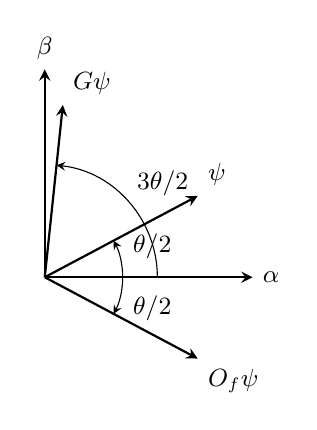
\begin{tikzpicture}[
        scale=2.2,
        >=stealth,
        every node/.style={font=\small}
    ]

        % Define angle
        \def\th{28}

        % Axes
        \draw[->, thick] (0,0) -- (1.2,0) node[right] {$\ket{\alpha}$};
        \draw[->, thick] (0,0) -- (0,1.2) node[above] {$\ket{\beta}$};

        % States
        \draw[->, thick] (0,0) -- ({cos(\th)},{sin(\th)}) 
            node[above right] {$\ket{\psi}$};

        \draw[->, thick] (0,0) -- ({cos(3*\th)},{sin(3*\th)}) 
            node[above right] {$G\ket{\psi}$};

        \draw[->, thick] (0,0) -- ({cos(-\th)},{sin(-\th)}) 
            node[below right] {$O_f\ket{\psi}$};

        % Upward theta/2 arc
        \draw[->] (0.45,0) arc[start angle=0,end angle=\th,radius=0.45];
        \node at (0.62,0.18) {$\theta/2$};

        % Downward theta/2 arc
        \draw[->] (0.45,0) arc[start angle=0,end angle={-\th},radius=0.45];
        \node at (0.62,-0.18) {$\theta/2$};

        % Larger arc for 3theta/2
        \draw[->] (0.65,0) arc[start angle=0,end angle={3*\th},radius=0.65];
        \node at (0.68,0.54) {$3\theta/2$};

    \end{tikzpicture}
    \caption{Geometric picture of a single Grover iterate in the plane spanned by $\ket{\alpha}$ and $\ket{\beta}$. The oracle $O_f$ reflects $\ket{\psi}$ across the $\ket{\alpha}$ axis, then the second operator $2\ketbra{\psi}{\psi}-I$ reflects $O_f\ket{\psi}$ across $\ket{\psi}$ axis. The net effect is a final rotation $G\ket{\psi}$, which is now closer to $\ket{\beta}$. Note that the angle $\theta$ has been greatly exaggerated for readability.}
    \label{fig:GroverGeometry}
    \end{figure}
    
    \item Starting from the state $\ket{\psi} = \cos\frac{\theta}{2}\ket{\alpha} + \sin\frac{\theta}{2}\ket{\beta}$ and applying $G$ gives us, after $k$ iterations,
    \[
        G^k\ket{\psi} = \cos\left( \frac{2k+1}{2}\theta\right)\ket{\alpha} + \sin\left( \frac{2k+1}{2}\theta\right)\ket{\beta}.
    \]
    To maximize the probability of obtaining an element in $B$ (i.e. getting a solution), we want that $\frac{2k+1}{2}\theta\ \approx \frac{\pi}{2}$. This leads us to choose $k = \lfloor \frac{\pi}{2\theta} - \frac{1}{2} \rceil$, where $\lfloor x \rceil$ denotes the rounding of $x$ to the nearest integer. Note that error is at most $\theta$, since if we are more than $\theta$ off from $\pi/2$ we would rotate further by another $\theta$. So smaller $M/N$ implies smaller $\theta$ implies higher precision.

    \item It is also wlog to assume $M \leq N/2$. In this situation, $\frac{\theta}{2} \geq \sin \frac{\theta}{2} = \sqrt{\frac{M}{N}}$, so
    \[
        k = \left\lfloor \frac{\pi}{2\theta} - \frac{1}{2} \right\rceil \leq \frac{\pi}{2\theta} \leq \left\lceil \frac{\pi}{4}\sqrt{\frac{N}{M}} \right\rceil,
    \]
    i.e. the number of Grover iterations required is $k = \mathcal{O}(\sqrt{\frac{N}{M}})$, a quadratic improvement over the $\mathcal{O}(\frac{N}{M})$ classical solution. If $M \geq N/2$, we simply double $N$ by introducing an extra qubit (i.e. $n \rightarrow n+1$) and extending $f$ such that the original marked items remain marked only when the ancilla is in the state $\ket{0}$.

    \item What have we done? We have effectively \textit{amplified} the probability of getting a solution, from $\sin^2\left(\frac{\theta}{2}\right)$ to $\sin^2\left(\frac{2k+1}{2}\theta \right) \approx 1$, by choosing $k$ appropriately. 


    
\end{enumerate}









